
El detector CMS, representado de manera esquem\'atica en la Figura~\ref{fig:CMS}, se localiza en uno de los puntos del acelerador LHC donde se hacen colisionar los haces de protones. Est\'a compuesto, de la zona m\'as interna a la m\'as externa, por un tracker de p\'ixeles y tiras (strips) de silicio para la detecci\'n de partículas cargadas con gran resoluci\'on espacial, un calor\'metro electromagn\'etico de cristal de tungstato (ECAL) para la medida de electrones y fotones principalmente, un calor\'imetro hadr\'onico constituido de material denso y absorbente (HCAL) especializado en la medida de hadrones, y finalmente, en la parte m\'as externa se encuentran las c\'amaras de muones. Entre el HCAL y las c\'amaras de muones se tiene un im\'an superconductor que alcanza un campo magn\'etico de 3.8 T, suficiente para curvar part\'iculas cargadas de muy alto momento y permitir una buena resoluci\'on en la medida del mismo.

\begin{figure}[h]
\centering
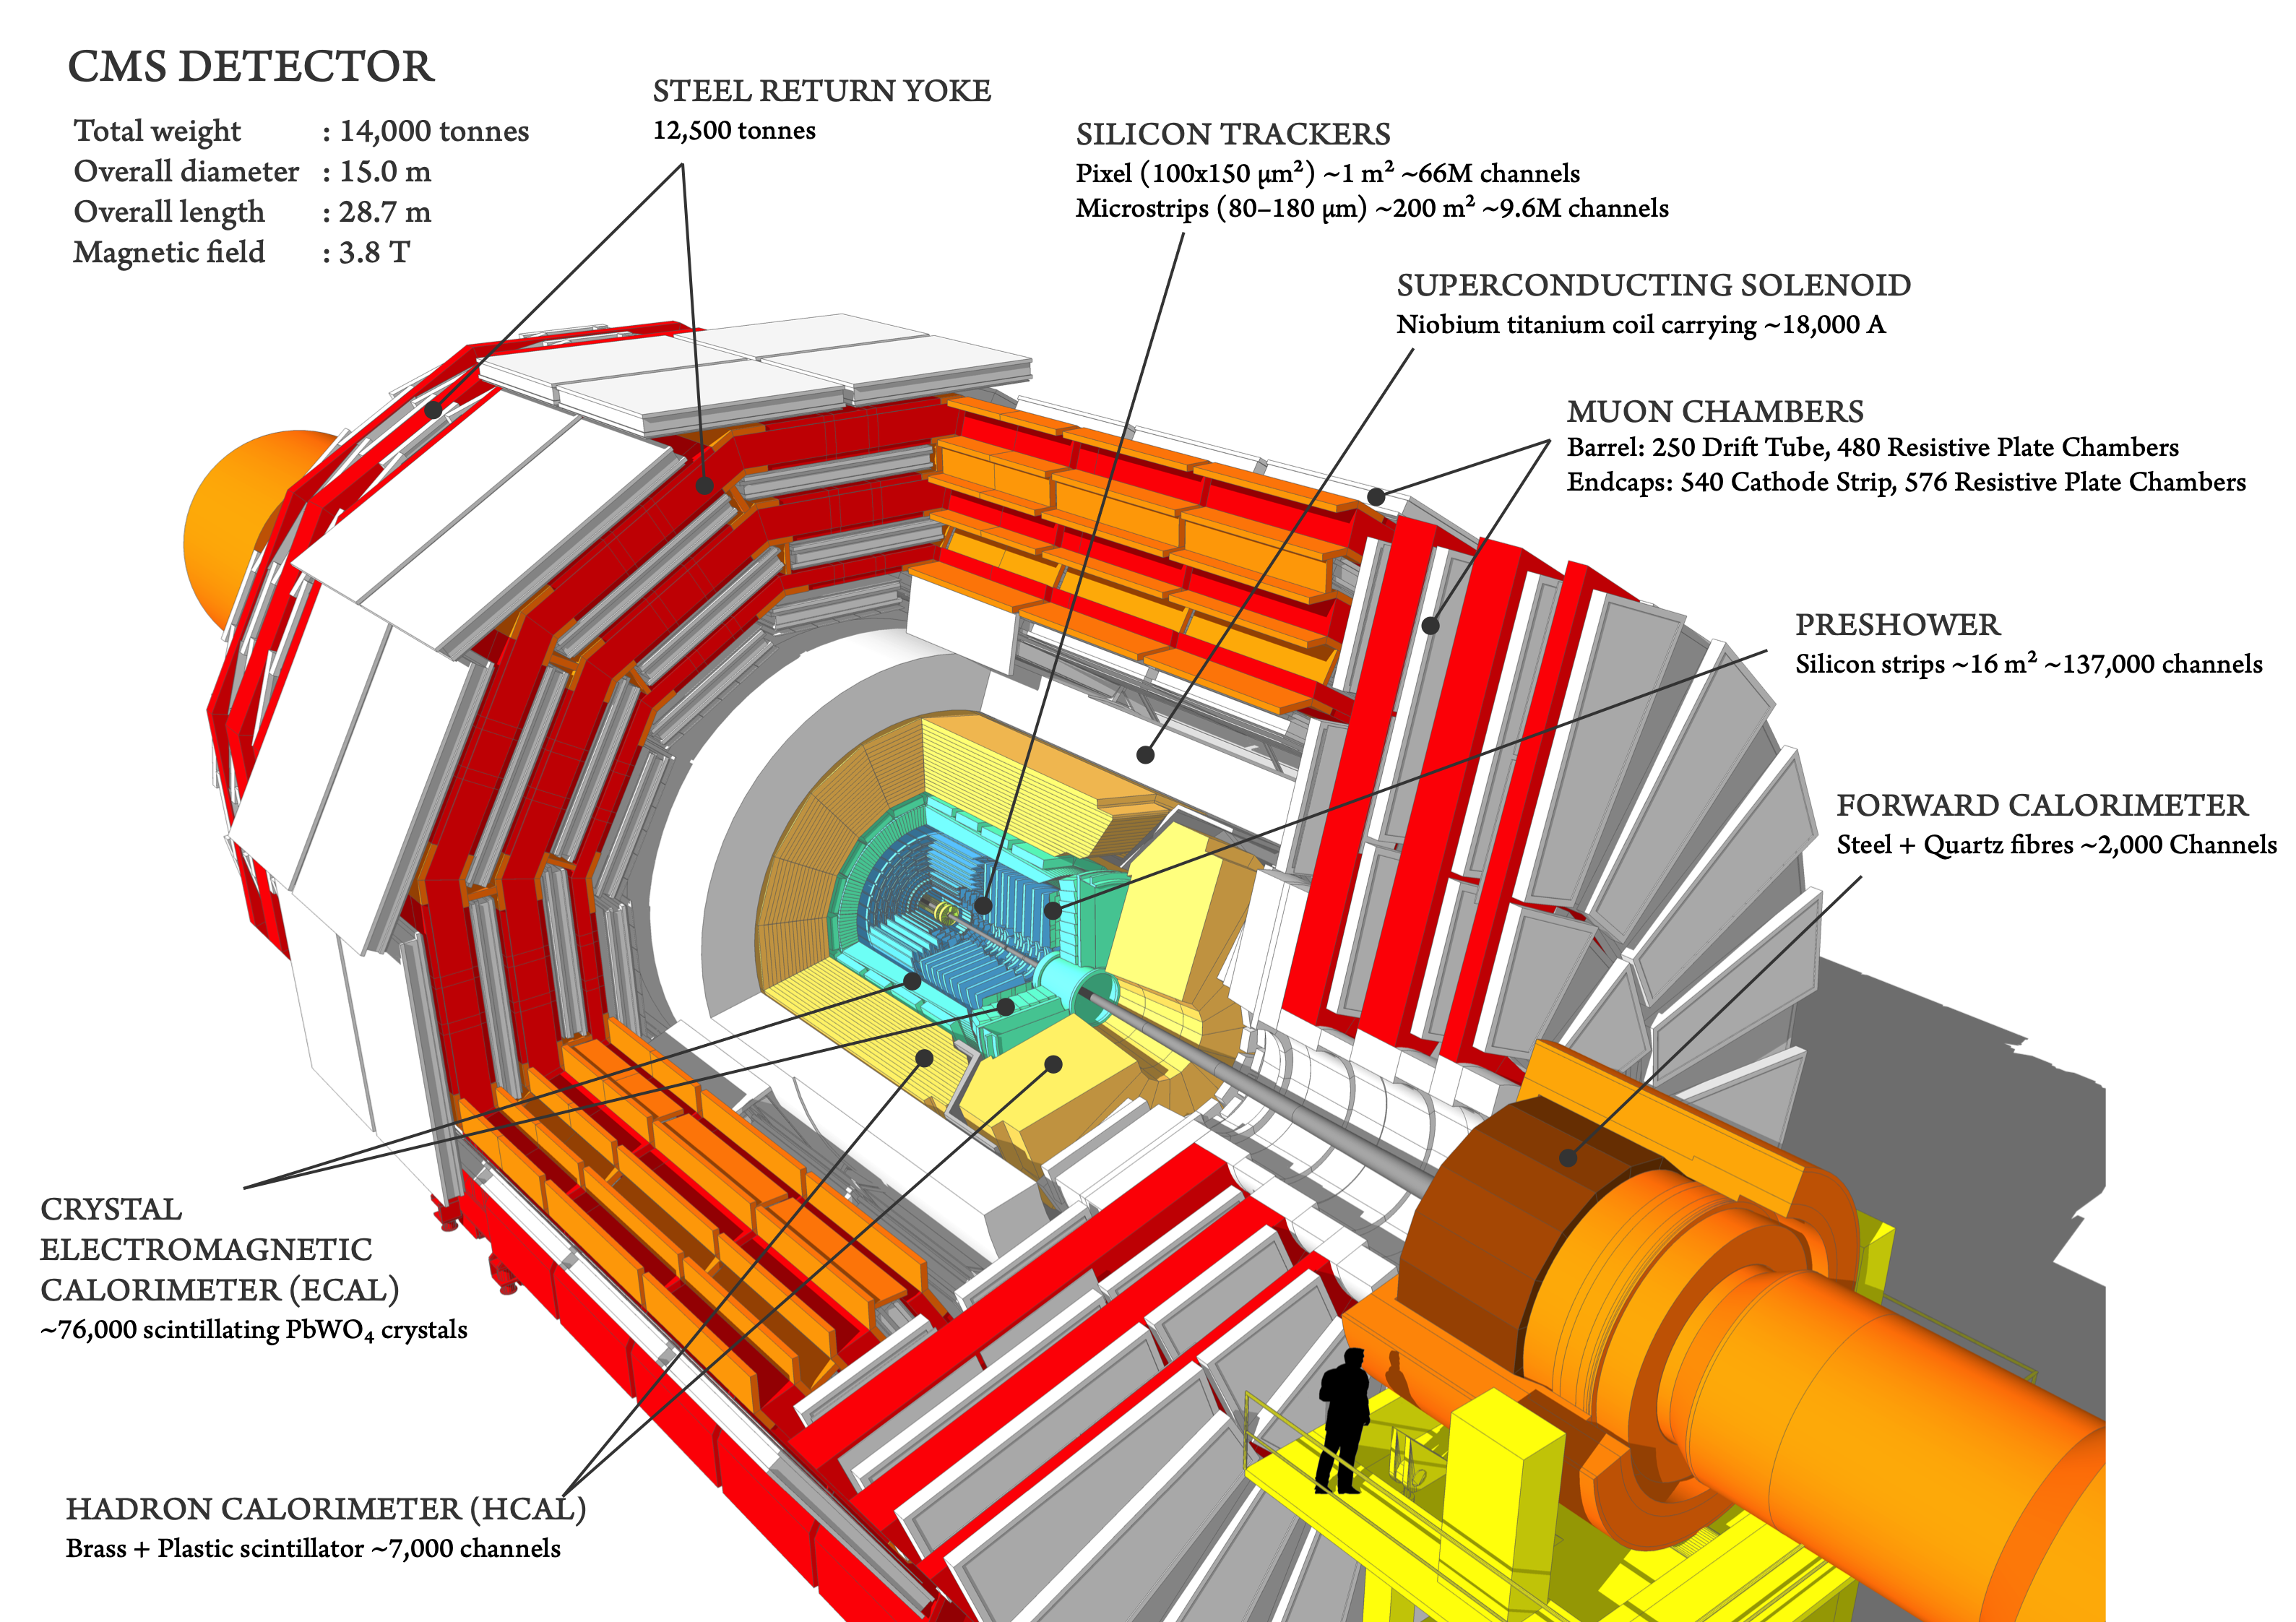
\includegraphics[width=0.80\textwidth]{figures/cms_160312_02.png}
\caption{Representaci\'on gr\'afica de las distintas partes del detector CMS. Imagen tomada de \cite{Sakuma:2665537}.}
\label{fig:CMS}        
\end{figure}

En cuanto a su geometr\'ia, el sistema de coordenadas aceptado tiene como origen el punto de colisi\'on, el eje y apunta verticalmente hacia arriba, el eje x radialmente desde el origen, y el eje z recorre la direcci\'on del haz (ver Figura~\ref{fig:CMS}). El \'angulo azimutal $\phi$ se mide a partir del eje x en el plano x-y transverso al haz, mientras que el \'angulo polar $\theta$ desde el eje z en el plano x-z. Otra variable angular importante que ser\'a utilizada en el an\'alisis por ser invariante bajo transformaciones de Lorentz en el eje z, es la pseudorrapidez $\eta$, que se define en funci\'on del \'angulo polar como:

\begin{equation}
  \eta = -\ln\left(\tan\dfrac{\theta}{2}\right)
\label{eq:eta}
\end{equation}


De esta manera, se suelen usar variables definidas en el plano transversal a la dirección del haz de partículas como el momento transverso $p_{T}$ o la energía transversa $E_{T}$. 

En este trabajo nos centraremos en la medida de los muones, que al ser part\'iculas cargadas dejan se\~nal en el tracker interno, no interaccionan apenas con el material denso de los calor\'imetros, y llegan a las c\'amaras de muones externas, situadas a unos cuatro metros del punto de colisi\'on. En las siguientes subsecciones se describir\'an dos de los subdetectores que componen las c\'amaras de muones que ser\'an utilizados en el an\'alisis: los Drift Tubes (DTs), y los Cathode Strip Chambers (CSCs).

\subsection{Drift Tubes: DTs}\label{sec:DTs}

Los drift tubes~\cite{DTperformance} cubren el barril de CMS ($\lvert \eta \rvert <$ 0.9). Cada tubo se compone de un hilo colector de carga cargado positivamente y est\'a lleno de gas, de manera que una part\'icula cargada a su paso por el tubo arranca electrones de los \'atomos del gas, que son atraidos el\'ectricamente y recolectados por el hilo conductor. De esta manera, a partir de la posici\'on en el hilo donde los electrones impactan y obteniendo la distancia del mu\'on al hilo se obtienen las coordenadas del paso del mu\'on por el tubo.

El subdetector completo consta de 250 c\'amaras, cada una de ellas con unas dimensiones en promedio de 2 x 2.5 m, formada por de tres capas con unos 60 tubos cada una repartidos en cuatro subcapas. Las c\'amaras en el barril se denotan como MBZ/N/S, donde Z=-2...+2 se corresponde con el n\'umero de rueda a lo largo del eje z, N=1...4 hace referencia al n\'umero de estaci\'on conc\'entrica en el plano xy, y S=1...12 al n\'umero de sector circular. En la Figura~\ref{fig:CMSsub} se representa gr\'aficamente la posici\'on espacial de las distintas c\'amaras.


\subsection{Cathode Strip Chambers: CSCs}\label{sec:CSCs}

Los cathode strip chambers~\cite{CSCperformance} cubren las tapas de CMS (1.2 $< \lvert \eta \rvert <$ 2.4). Su funcionamiento es similar a las DTs, en el sentido de que tambi\'en son c\'amaras de gas que utilizan la deriva de los electrones hacia un \'anodo para determinar la posici\'on del mu\'on que las atraviesa.

El subdetector completo de las CSC contiene 540 c\'amaras en total, y est\'a compuesto de anillos de c\'amaras trapezoidales de hasta 3.4 m de largo y 1.5 m de ancho, colocadas en ocho discos, cuatro en cada tapa. Las c\'amaras se denotan espacialmente como ME$\pm$S/R, donde el signo indica en qu\'e tapa de CMS se encuentra, S=1...4 hace referencia al n\'umero de estaci\'on, paralelas en el eje z (ver Figura~\ref{fig:CMSsub}), y R se corresponde con el n\'umero de anillo, conc\'entricos en el plano xy. En la Figura~\ref{fig:CSC_MEm1} se muestra una imagen real de la rueda ME-1, con sus tres anillos conc\'entricos en el plano xy. \\

\begin{figure}[h]
\centering
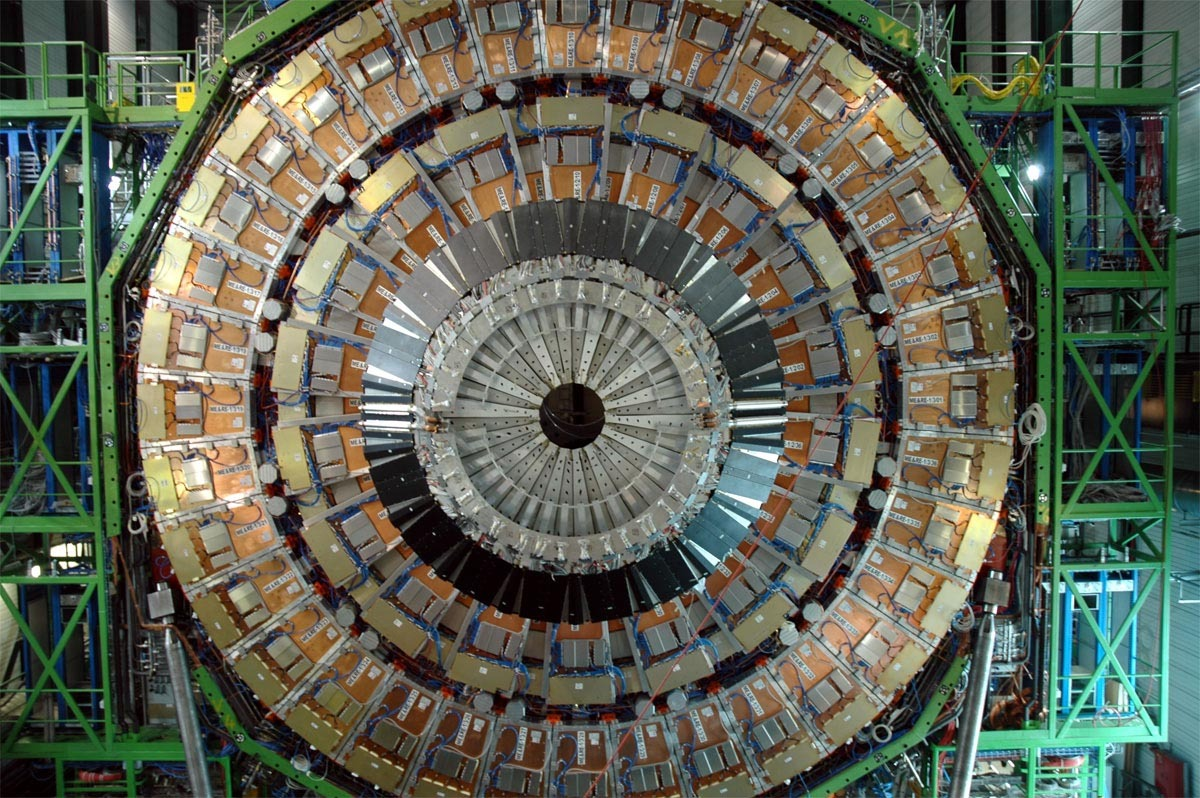
\includegraphics[width=0.60\textwidth]{figures/CSC_MEm1.jpg}
\caption{Foto completa de la estaci\'on ME-1. Imagen tomada de \cite{Breedon:1431505}.}
\label{fig:CSC_MEm1}        
\end{figure}


\begin{figure}
\centering
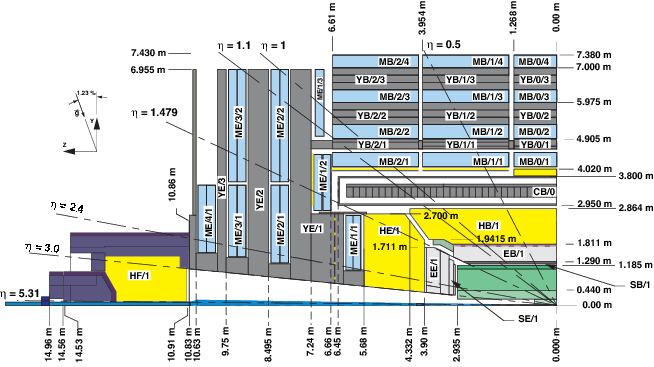
\includegraphics[width=0.8\textwidth]{figures/CMSview1.png}
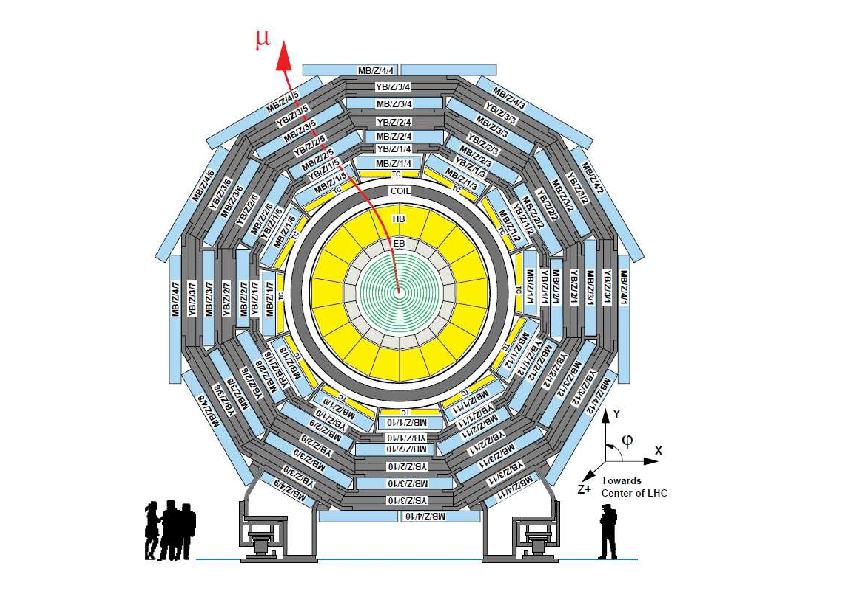
\includegraphics[width=0.8\textwidth]{figures/CMSview.png}
\caption{Vista esquem\'atica del detector CMS. Arriba: vista longitudinal de un cuarto del detector. Abajo: vista transversal en $z = 0$. Ambas figuras han sido tomadas de \cite{DTperformance}.}
\label{fig:CMSsub}
\end{figure}


Las c\'amaras DT y CSC se componen de varias capas, y las se\~nales o hits que dejan los muones a su paso se reconstruyen en cada cada de ellas. A partir de estos hits por c\'amara, se construyen trazas rectas denominadas segmentos dentro de cada c\'amara DT o CSC. 
